\chapter{Appendix}\label{ch_appendix}

\section{Approximation Algorithm for Optimal Multidimensional Auctions}\label{appendix:algo}

I adopt and improve the original finite-dimensional approximation algorithm of \autocite{belloni2010multidimensional} by focusing on local and downward-sloping incentive-compatibility constraint (ICC) violations. Although these local constraints are often violated in this approximate setting, I drastically reduce the number of times \textit{all} incentive-compatible constraints need to be checked.

In order to approximate an optimal solution to \ref{eq_opt_interim}, I discretize the type space $X$. Let $T$ denote a positive integer that controls the granularity of the discretization. For each $j \in J$, let $X_T(j)$ denote the discretization of the interval $[\underline{x}_j,\overline{x}_j]$ given by $X_T(j) = \{\underline{x}_j, \underline{x}_j + \epsilon, \underline{x}_j + 2\epsilon, \dots, \overline{x}_j\}$ where $\epsilon = \min_{j \in J} \{(\overline{x}_j - \underline{x}_j) / T\}$. Our discretized version of the type space $X$ is given by $X_T := \prod_{j \in J} X_T(j)$. Furthermore, I define a probability density function on $X_T$ by setting $\hat{f}(v) = f(v) / (\sum_{t \in X_T} f(t))$. I thus obtain a linear program which is a finite-dimensional approximation of \ref{eq_opt_interim} for each $T > 0$ by replacing $X$ with $X_T$.

\begin{figure}[t]
    \begin{center}
    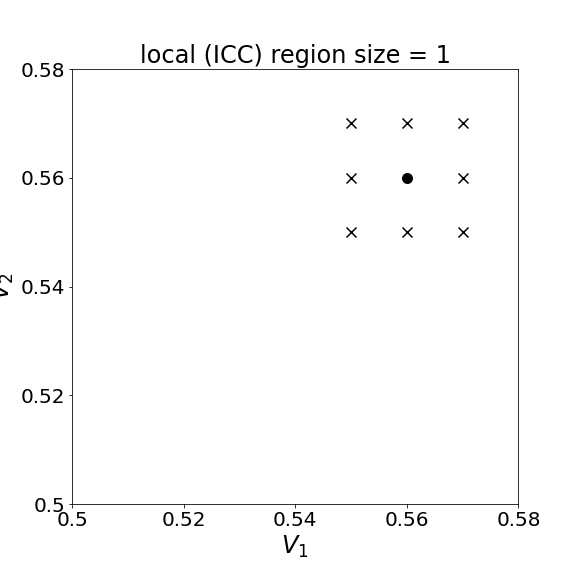
\includegraphics[width=0.3\textwidth]{images/local_size_1.png}
    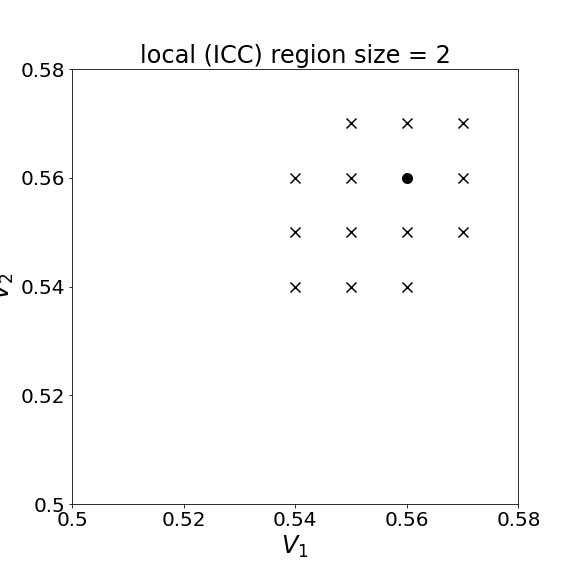
\includegraphics[width=0.3\textwidth]{images/local_size_2.png}
    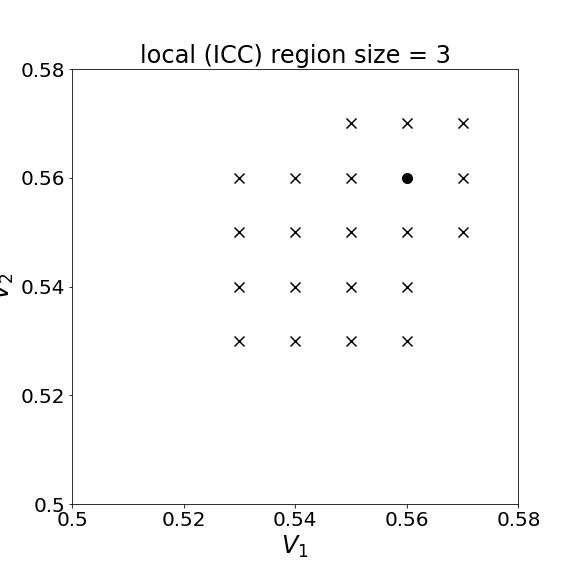
\includegraphics[width=0.3\textwidth]{images/local_size_3.png}
    \end{center}
    
    \vspace{1mm}
    \raggedright{\small {\sc Figure \refstepcounter{fig}\thefig\label{fig:sim1}:} We iteratively grow the local region of the discretized type space checked for downwards-sloping constraint violations. Notice that immediately adjacent (ICC) constraints are always checked ($\times$) when the local region increases in size around a point ($\bullet$).}
\end{figure}


Belloni et al. \autocite*{belloni2010multidimensional} use a plane-putting algorithm which works with a randomly chosen subset of incentive-compatibility (ICC) and Border (B) constraints at each iteration. They provide an efficient reduction in the growth in $T$ of the Border constraints (B) from $O(2^{T^J})$ to $O(T^J \log(T^J))$ \autocite[Lemma 10]{belloni2010multidimensional}. We adopt their solution to checking (B) constraints; however, our approach to checking (ICC) constraints involves iteratively growing the `local' region of the type space around each point $v$ in the discretized set of types $V_T$. We do two things. First, all the immediately adjacent points in the discretized type space are always checked for incentive compatibility. Secondly, downwards-sloping points in the discretized type space are also checked. Furthermore, the downwards-sloping region of the type space grows until all (ICC) constraints are ultimately satisfied. This procedure is illustrated visually in Figure \ref{fig:sim1}. Thus, for a fixed-size local region around each point in the discretized type space, we first satisfy \textit{local} (ICC) and (B) constraints as in the iterative plane-cutting algorithm of \autocite{belloni2010multidimensional}. Then we run the separation oracle with \textit{all} (ICC) and (B) constraints. We then restart the solver with any previously violated constraints, this time increasing the size of the local region around each point in the discretized type space. This procedure iterates until no constraints are violated. This modified version of \autocite{belloni2010multidimensional}'s algorithm is described in Algorithm \ref{alg:1}.

\begin{figure}[t]
  \centering
  \begin{minipage}{.7\linewidth}
    \begin{algorithm}[H]
    \caption{Iterative plane-cutting algorithm with local and downwards-sloping (ICC) constraints}\label{alg:1}
    \SetAlgoLined
    % \KwData{$x=1$}
    % \KwResult{$y = x^n$}
    % $\text{local_size} = 1$\;
    $L = 1, S = \emptyset, A = \emptyset, \overline{OPT} = \infty$\;
    \texttt{violated\_any\_icc} $\gets $ TRUE\; 
    \While{\texttt{violated\_any\_icc}}{
        \texttt{violated\_local\_icc} $\gets$ TRUE\; 
        \While{\texttt{violated\_local\_icc}}{
          $k = 1, A^k = A, S^k = S$\;
          Solve the linear program associated with $S^k$. Let $OPT^k$ denote the optimal value.\;
          Solve the separation oracle using only local (ICC) constraints in region $L$. Let $A^k$ denote all violated local (ICC) and (B) constraints.\;
          \If{$A^k = \emptyset$}{
            \texttt{violated\_local\_icc} $\gets$ FALSE\;
            Break\;
          }
          Select a subset $I^k \subset S^k$ of inactive (ICC) and (B) constraints\;
          \eIf{$OPT^k < \overline{OPT}$}{
            $S^{k+1} \gets (S^k \setminus I^k) \cup A^k \cup A$\;
            $\overline{OPT} \gets OPT^k$\;
          }{
            $S^{k+1} \gets S^k \cup A^k \cup A$\;
          }
          $k \gets k+1$\;
        }
        Solve the separation oracle using all (ICC) constraints. Let $A^*$ denote all violated (ICC) constraints.\;
        \If{$A^* = \emptyset$}{
            \texttt{violated\_any\_icc} $\gets$ FALSE\;
            Break\;
        }
        $A \gets A \cup A^*$\;
        $S \gets S^k$\;
        $L \gets L + 1$\;
    }
    \end{algorithm}
  \end{minipage}
\end{figure}

Our algorithm\footnote{For more details see: \url{https://github.com/jmemich/optimal-auction-multidim}} is written in Python 3.10 and uses Google's open source linear programming solver `GLOP' available in their \texttt{or-tools} package \autocite{ortools}.

\section{Census Non-Response Calculations}\label{appendix_census_calc}

The 2020 census post-enumeration survey data can be found in the US Census data tables\footnote{\url{https://data.census.gov/table}}, where the `Net Coverage Error for the Household Population in the United States by Race and Hispanic Origin' is given by the variable \textbf{C\_RACEHISUS} and the net coverage error is estimated at -4.99\%. The data for the 2010 US Census are not available on the census data tables, however, the official estimated net undercount of Hispanics was -1.54\% \autocite[p1]{census2010coverage}.


